
\documentclass[12pt,journal,compsoc]{IEEEtran}


% *** CITATION PACKAGES ***
%
\ifCLASSOPTIONcompsoc
  % IEEE Computer Society needs nocompress option
  % requires cite.sty v4.0 or later (November 2003)
  % \usepackage[nocompress]{cite}
\else
  % normal IEEE
  % \usepackage{cite}
\fi


% *** GRAPHICS RELATED PACKAGES ***
%
\ifCLASSINFOpdf
  % \usepackage[pdftex]{graphicx}
  % declare the path(s) where your graphic files are
  % \graphicspath{{../pdf/}{../jpeg/}}
  % and their extensions so you won't have to specify these with
  % every instance of \includegraphics
  % \DeclareGraphicsExtensions{.pdf,.jpeg,.png}
\else
  % or other class option (dvipsone, dvipdf, if not using dvips). graphicx
  % will default to the driver specified in the system graphics.cfg if no
  % driver is specified.
  % \usepackage[dvips]{graphicx}
  % declare the path(s) where your graphic files are
  % \graphicspath{{../eps/}}
  % and their extensions so you won't have to specify these with
  % every instance of \includegraphics
  % \DeclareGraphicsExtensions{.eps}
\fi

\providecommand{\PSforPDF}[1]{#1}


% NOTE: PDF hyperlink and bookmark features are not required in IEEE
%       papers and their use requires extra complexity and work.
% *** IF USING HYPERREF BE SURE AND CHANGE THE EXAMPLE PDF ***
% *** TITLE/SUBJECT/AUTHOR/KEYWORDS INFO BELOW!!           ***
\newcommand\MYhyperrefoptions{bookmarks=true,bookmarksnumbered=true,
pdfpagemode={UseOutlines},plainpages=false,pdfpagelabels=true,
colorlinks=true,linkcolor={black},citecolor={black},pagecolor={black},
urlcolor={black},
pdftitle={Bare Demo of IEEEtran.cls for Computer Society Journals},%<!CHANGE!
pdfsubject={Typesetting},%<!CHANGE!
pdfauthor={Michael D. Shell},%<!CHANGE!
pdfkeywords={Computer Society, IEEEtran, journal, LaTeX, paper,
             template}}%<^!CHANGE!



% correct bad hyphenation here
\hyphenation{op-tical net-works semi-conduc-tor}


\begin{document}
%
% paper title
% can use linebreaks \\ within to get better formatting as desired
\title{Bare Advanced Demo of IEEEtran.cls\\ for Computer Society Journals}
%
%


\author{Michael~Shell,~\IEEEmembership{Member,~IEEE,}
        John~Doe,~\IEEEmembership{Fellow,~OSA,}
        and~Jane~Doe,~\IEEEmembership{Life~Fellow,~IEEE}% <-this % stops a space
\IEEEcompsocitemizethanks{\IEEEcompsocthanksitem M. Shell is with the Department
of Electrical and Computer Engineering, Georgia Institute of Technology, Atlanta,
GA, 30332.\protect\\
% note need leading \protect in front of \\ to get a newline within \thanks as
% \\ is fragile and will error, could use \hfil\break instead.
E-mail: see http://www.michaelshell.org/contact.html
\IEEEcompsocthanksitem J. Doe and J. Doe are with Anonymous University.}% <-this % stops a space
\thanks{Manuscript received April 19, 2005; revised January 11, 2007.}}





% The paper headers
\markboth{Journal of \LaTeX\ Class Files,~Vol.~6, No.~1, January~2007}%
{Shell \MakeLowercase{\textit{et al.}}: Bare Advanced Demo of IEEEtran.cls for Journals}
% The only time the second header will appear is for the odd numbered pages
% after the title page when using the twoside option.
% 
% *** Note that you probably will NOT want to include the author's ***
% *** name in the headers of peer review papers.                   ***
% You can use \ifCLASSOPTIONpeerreview for conditional compilation here if
% you desire.






% for Computer Society papers, we must declare the abstract and index terms
% PRIOR to the title within the \IEEEcompsoctitleabstractindextext IEEEtran
% command as these need to go into the title area created by \maketitle.
\IEEEcompsoctitleabstractindextext{%
\begin{abstract}
%\boldmath
The abstract goes here.
\end{abstract}
% IEEEtran.cls defaults to using nonbold math in the Abstract.
% This preserves the distinction between vectors and scalars. However,
% if the journal you are submitting to favors bold math in the abstract,
% then you can use LaTeX's standard command \boldmath at the very start
% of the abstract to achieve this. Many IEEE journals frown on math
% in the abstract anyway. In particular, the Computer Society does
% not want either math or citations to appear in the abstract.

% Note that keywords are not normally used for peerreview papers.
\begin{IEEEkeywords}
Computer Society, IEEEtran, journal, \LaTeX, paper, template.
\end{IEEEkeywords}}


% make the title area
\maketitle


% To allow for easy dual compilation without having to reenter the
% abstract/keywords data, the \IEEEcompsoctitleabstractindextext text will
% not be used in maketitle, but will appear (i.e., to be "transported")
% here as \IEEEdisplaynotcompsoctitleabstractindextext when compsoc mode
% is not selected <OR> if conference mode is selected - because compsoc
% conference papers position the abstract like regular (non-compsoc)
% papers do!
\IEEEdisplaynotcompsoctitleabstractindextext
% \IEEEdisplaynotcompsoctitleabstractindextext has no effect when using
% compsoc under a non-conference mode.


% For peer review papers, you can put extra information on the cover
% page as needed:
% \ifCLASSOPTIONpeerreview
% \begin{center} \bfseries EDICS Category: 3-BBND \end{center}
% \fi
%
% For peerreview papers, this IEEEtran command inserts a page break and
% creates the second title. It will be ignored for other modes.
\IEEEpeerreviewmaketitle


\section{Introduction}

\IEEEPARstart{T}{his} demo file is intended to serve as a ``starter file''
for IEEE Computer Society journal papers produced under \LaTeX\ using
IEEEtran.cls version 1.7 and later.
% You must have at least 2 lines in the paragraph with the drop letter
% (should never be an issue)
I wish you the best of success.

\hfill mds
 
\hfill January 11, 2007


\section{Graph Based Indoor Tracking}
%!TEX root = ../bare_adv.tex
\subsection{Introduction}
When talking about indoor positioning, a Graph-based Model~\cite{Jensen:2009:GMB:1590953.1591000} describes the topology of e.g. a floor plan of the indoor area. 
This area may be a complex area with several rooms, levels, doors, hallways etc. 
The Graph-based Model therefore represents the connectivity and accessibility of the area, representing each room as a vertex and each connection as an edge. 

By representing the area using a Graph-based Model, it is possible to apply indoor tracking of the people that are inside the area, using various wireless technologies (like bluetooth, Wi-Fi, RFID etc.) by logging the movement of the people or objects we want to track.

%A Graph-based Model can be applied, as it does not differ between the actual floor plan and the abstract model, hence why using an abstract model provides a equally correct positioning data. 

\subsection{Explained}
There are two kinds of Graph-based Models that describes the the topology of a floor plan. 
The first is the Connectivity Graph which describes how rooms, hallways, stairs etc. are connected to each other. 
The second is the Accessibility Graph which takes the actual accessibility of a room into account. 
These two will be described in the following sections. 


\subsubsection{ \quad Connectivity Graph}
Both the Connectivity graph and the Accessibility Graph are based on a base-graph, which is constructed based on the actual floor plan. 

\begin{figure}[H]%
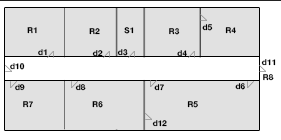
\includegraphics{images/floorplan.png}%
\caption{Floor plan of a building. Inspired from~\cite{Jensen:2009:GMB:1590953.1591000}}%
\label{fig:floortplan}%
\end{figure}%

Figure \ref{fig:floortplan} shows the floor plan that forms the basis of the examples of the Connectivity graph and the Accessibility graph. 
It contains 7 rooms, labeled $R1 - R7$, one staircase labeled $S1$, a hallway and 12 doors labeled $d1-d12$. \\

In the Connectivity graph, each separate partitioning of the floor plan (rooms, staircases, hallways etc.) are represented as vertices, while the connectivity of these (doors, windows, hatches etc.) are represented as the edges.
E.g. if two rooms are connected by a door, each room will be represented in the base-graph as a vertex, while the door is represented as an undirected edge. 
The Connectivity graph representing the floor plan in Figure \ref{fig:floortplan} is shown in Figure \ref{fig:connectivitygraph} below. 

\begin{figure}[H]%
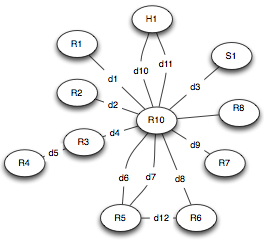
\includegraphics{images/connectivitygraph.png}%
\caption{Connectivity Graph of the floor plan in Figure \ref{fig:floortplan}.}%
\label{fig:connectivitygraph}%
\end{figure}%

Figure \ref{fig:connectivitygraph} shows how the rooms and hallways in Figure \ref{fig:floortplan} are connected by doors. 
The Connectivity graph itself is a labeled, undirected multi-graph that is defined by the following triple: \\

\begin{equation}
G_{connection} = (V, E_d, \Sigma_{door})
\end{equation}
In this triple, $V$ is the set of vertices in in the Graph. 
$E_d$ is the set of edges in the Graph, where any edge in $E_d$ is a pair consisting of $({v_i, v_j}, k)$ such that $v_i, v_j \in V$ and $k \in \Sigma_{door}$.
Finally, $\Sigma_{door}$ is a set of edge labels that represent the connections. 

However, it does not make much sense to look at the Connectivity Graph alone when talking about indoor positioning and tracking. 
To be able to track movement, information about the accessibility of each vertex must also be available. 

\subsubsection{ \quad Accessibility Graph}
There may be situations where a connection does not mean that you have access through that connection.
It can be air-port security or subway ententes that are either entries or exits, which allows one-way movement only.
To take this into account, the Accessibility graph is used. 
The Accessibility graph for the floor plan in Figure \ref{fig:floortplan} is shown in Figure \ref{fig:accesibbilitygraph} below.

\begin{figure}[H]%
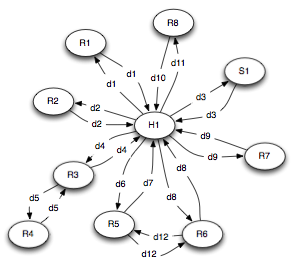
\includegraphics{images/accessibilitygraph.png}%
\caption{Accesibility graph of the floor plan in Figure \ref{fig:floortplan}.} % and the connectivity graph in Figure \ref{fig:floortplan}.}%
\label{fig:accesibbilitygraph}%
\end{figure}%

Figure \ref{fig:accesibbilitygraph} shows the accessibility graph..
It can be seen that door $d10$ only allows entrance from outside and into the Hall, while door $d11$ only allows exit from the Hall.
The Accessibility graph is a labeled, directed graph and constructed to represent possible movement patterns in the area. \\

An Accessibility graph named $G_{access}$ is given by the triple: 

\begin{equation}
G_{access} = (V, E, \Sigma_{door}, l_e)
\end{equation} 

where $V$ is the set of vertices, $E$ is the set of directed edges, having $E = {\langle v_i, v_j \rangle | v_i, v_j \in V \not v_i != v_j}$ and finally $l_e$ is a function that maps edges to subsets of the doors, having $l_e : E \rightarrow 2^{\Sigma_{door}}$. \\

These graphs provide an abstract representation of the floor plan, which -- combined with the previously mentioned logging -- will allow for indoor movement tracking and indoor positioning. 

%\IEEEPARstart{T}{his} demo file is intended to serve as a ``starter file''
%for IEEE Computer Society journal papers produced under \LaTeX\ using
%IEEEtran.cls version 1.7 and later.
% You must have at least 2 lines in the paragraph with the drop letter
% (should never be an issue)
%I wish you the best of success.
%\hfill mds
%\hfill January 11, 2007

\subsection{Logging of Sensor Data}
When a reader detects a object it records a log. 
A reading is of the following format \textless $readerID,objectID,timestamp$ \textgreater.
The \textit{readerID} is the identity of the reader, \textit{objectID} is the identity of the object which is in the range of the reader, and the \textit{timestamp} t is the time where the reader detected the object.
This recording is done at a given sampling rate. 
The same object might be recorded several times by the same reader in a row. 
A reader creates a log for each object that is in the vicinity of the reader thus there can be several logs with the same timestamp.

From this log data on-line and off-line outputs are generated~\cite{Jensen:2009:GMB:1590953.1591000}.
All data from the readers are continuously streamed to a database that is responsible for maintaining the data.
If a object enters or leave the range of a reader an on-line output is generated, this have the form
\begin{align}
\textless readerID,objectID,t,flag \textgreater 
\end{align}

where \textit{flag} is "`START"' or "`END"' respectively. 
%When the object is no longer detected by the reader an output is generated. 
Note that when a object in no longer detected by the reader  the \textit{flag} is set to "`END"' and the timestamp is the last \textit{t} where the object was within the vicinity.
A second output is generated when it have the form 
\begin{align}
\textless\textit{$readerID,objectID,t_{first},t_{last}$}\textgreater
\end{align}
These two outputs are later used in online and offline tracking which we cover in Section~\ref{sub:online} and Section~\ref{sub:offline}.

 

\section{Introduction}

\IEEEPARstart{T}{his} demo file is intended to serve as a ``starter file''
for IEEE Computer Society journal papers produced under \LaTeX\ using
IEEEtran.cls version 1.7 and later.
% You must have at least 2 lines in the paragraph with the drop letter
% (should never be an issue)
I wish you the best of success.

\hfill mds
 
\hfill January 11, 2007


% Computer Society journal papers do something a tad strange with the very
% first section heading (almost always called "Introduction"). They place it
% ABOVE the main text! IEEEtran.cls currently does not do this for you.
% However, You can achieve this effect by making LaTeX jump through some
% hoops via something like:
%
%\ifCLASSOPTIONcompsoc
%  \noindent\raisebox{2\baselineskip}[0pt][0pt]%
%  {\parbox{\columnwidth}{\section{Introduction}\label{sec:introduction}%
%  \global\everypar=\everypar}}%
%  \vspace{-1\baselineskip}\vspace{-\parskip}\par
%\else
%  \section{Introduction}\label{sec:introduction}\par
%\fi
%
% Admittedly, this is a hack and may well be fragile, but seems to do the
% trick for me. Note the need to keep any \label that may be used right
% after \section in the above as the hack puts \section within a raised box.



% The very first letter is a 2 line initial drop letter followed
% by the rest of the first word in caps (small caps for compsoc).
% 
% form to use if the first word consists of a single letter:
% \IEEEPARstart{A}{demo} file is ....
% 
% form to use if you need the single drop letter followed by
% normal text (unknown if ever used by IEEE):
% \IEEEPARstart{A}{}demo file is ....
% 
% Some journals put the first two words in caps:
% \IEEEPARstart{T}{his demo} file is ....
% 
% Here we have the typical use of a "T" for an initial drop letter
% and "HIS" in caps to complete the first word.

\section{Fingerprint Based Indoor Tracking}




\section{Discussion}









\appendices

%%%%%%%%%%%%%%%%%
%Make real bibtex setup
%%%%%%%%%%%%%%%%%

\section{Proof of the First Zonklar Equation}
Appendix one text goes here.

% you can choose not to have a title for an appendix
% if you want by leaving the argument blank
\section{}
Appendix two text goes here.


% use section* for acknowledgement
\ifCLASSOPTIONcompsoc
  % The Computer Society usually uses the plural form
  \section*{Acknowledgments}
\else
  % regular IEEE prefers the singular form
  \section*{Acknowledgment}
\fi


The authors would like to thank...


% Can use something like this to put references on a page
% by themselves when using endfloat and the captionsoff option.
\ifCLASSOPTIONcaptionsoff
  \newpage
\fi




\begin{thebibliography}{1}

\bibitem{IEEEhowto:kopka}
H.~Kopka and P.~W. Daly, \emph{A Guide to {\LaTeX}}, 3rd~ed.\hskip 1em plus
  0.5em minus 0.4em\relax Harlow, England: Addison-Wesley, 1999.

\end{thebibliography}

% biography section
% 
% If you have an EPS/PDF photo (graphicx package needed) extra braces are
% needed around the contents of the optional argument to biography to prevent
% the LaTeX parser from getting confused when it sees the complicated
% \includegraphics command within an optional argument. (You could create
% your own custom macro containing the \includegraphics command to make things
% simpler here.)
%\begin{biography}[{\includegraphics[width=1in,height=1.25in,clip,keepaspectratio]{mshell}}]{Michael Shell}
% or if you just want to reserve a space for a photo:

\begin{IEEEbiography}{Michael Shell}
Biography text here.
\end{IEEEbiography}

% if you will not have a photo at all:
\begin{IEEEbiographynophoto}{John Doe}
Biography text here.
\end{IEEEbiographynophoto}

% insert where needed to balance the two columns on the last page with
% biographies
%\newpage

\begin{IEEEbiographynophoto}{Jane Doe}
Biography text here.
\end{IEEEbiographynophoto}

% You can push biographies down or up by placing
% a \vfill before or after them. The appropriate
% use of \vfill depends on what kind of text is
% on the last page and whether or not the columns
% are being equalized.

%\vfill

% Can be used to pull up biographies so that the bottom of the last one
% is flush with the other column.
%\enlargethispage{-5in}



% that's all folks
\end{document}


